\chapter{LCD-näyttö}
\section{LCD-näytön kytkentä}\label{sec:lcd}

\begin{minipage}{0.5\textwidth}
\begin{tcolorbox}[colback=lime!10,title=Tarvikkeet, colbacktitle=green!10,coltitle=black]
\begin{itemize}
    \item Koekytkentälevy
    \item Arduino UNO 
    \item Potentiometri
    \item Hyppylankoja
    \item Vastus 220$\Omega$: 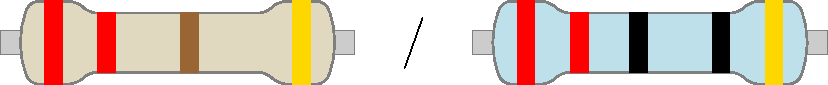
\includegraphics[width=0.5\textwidth]{kuvat/220.pdf}
    \item LCD-näyttö
\end{itemize}
\end{tcolorbox}
\end{minipage}
\begin{minipage}{0.5\textwidth}
\begin{tcolorbox}[colback=blue!10,title=Piirin toiminta,colbacktitle=purple!90]
Tutustutaan LCD-näytön käyttämiseen. Kirjoitetaan oma viesti näytölle. Potentiometrin käyttäminen ja sen avulla näytön kirkkauden säätäminen.
\end{tcolorbox}
\end{minipage}

\begin{tcolorbox}[colback=red!10,colbacktitle=red,title=HUOM!]
Aina kun rakennat tai muutat piiriä, pidä Arduino irrotettuna tietokoneesta! 
\tcblower
Huomaa, että LCD-näytön kytkemiseen tarvitaan useita hyppylankoja ja se vaatii tarkkuutta!
\end{tcolorbox}

\begin{tcolorbox}[title=Potentiometrin kytkeminen,colback=blue!10,colbacktitle=purple!90]
Potentiometri on säädettävä vastus, jossa on kolme jalkaa, kaksi toisella puolella ja yksi toisella. Se kytketään uran ylitse, niin että kaksi jaloista ovat toisella puolella ja yksi toisella puolella. Potentiometrin mukana tulee valkoinen säätönuppi, jolla vastuksen arvoa voidaan säädellä pyörittämällä nuppia. 

\begin{minipage}{0.8\textwidth}
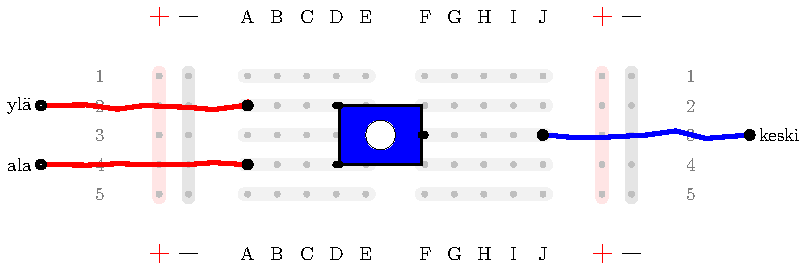
\includegraphics[width=\textwidth]{kuvat/kuva17.pdf}
\end{minipage}%
\begin{minipage}{0.2\textwidth}
Piirrustusmerkki:

\begin{circuitikz} 
\draw (0,0) node[left] {ylä} to[american potentiometer,n=mypot] ++(0,-2) node[right] {ala} (mypot.wiper) to[short] ++(1,0) node[above] {keski};
\end{circuitikz}
\end{minipage}

Mitattaessa vastuksen arvoa välillä ylä-ala, vastuksen arvo pysyy vakiona. Jos taas käytetään vastusta välillä ylä-keski tai keski-ala, vastuksen arvoa voidaan muuttaa pyörittämällä säätönuppia.
\end{tcolorbox}

\clearpage
Kytketään näyttöön tarvittavat asiat osissa koekytkentälevylle. Ole tarkkana rivien kanssa!

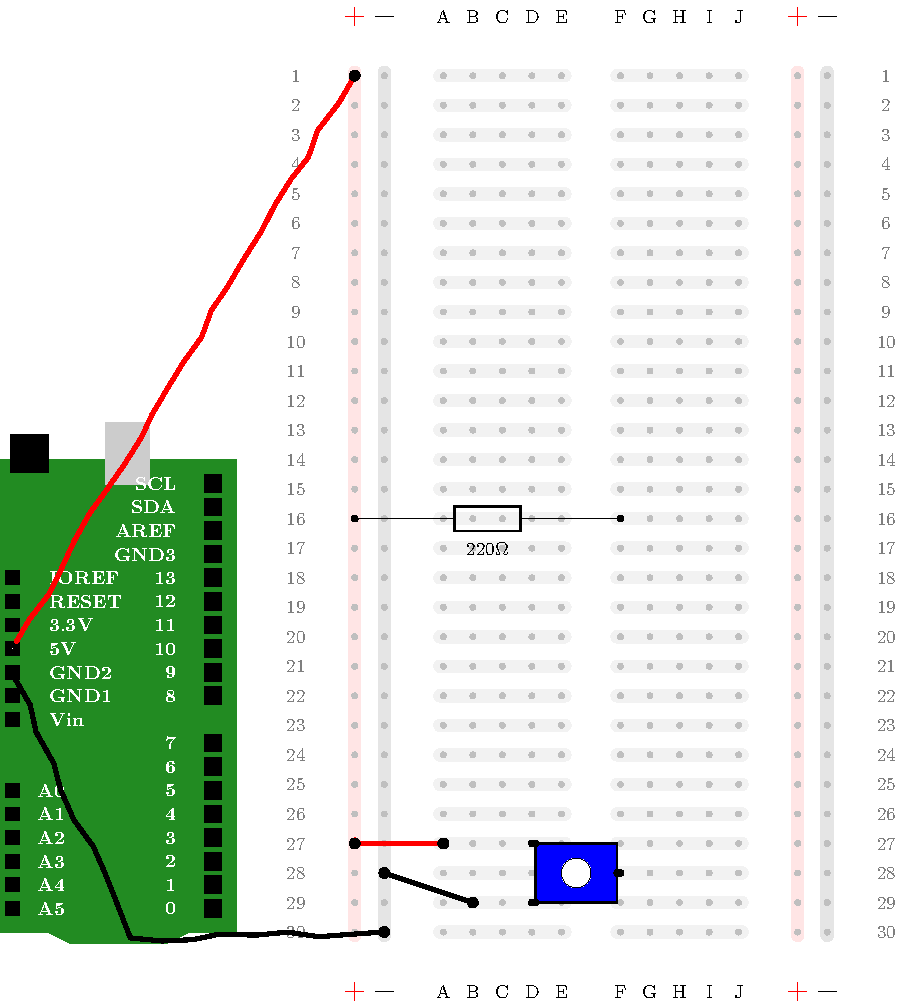
\includegraphics[width=0.95\textwidth]{kuvat/kuva19.pdf}

Kytketään ensin potentiometri pisteisiin D27, D29 ja F28. Kytke rivi 27 vasen puoli käyttöjännitteeseen (punainen + rivi) ja rivi 29 vasen puoli maahan. Kytketään sitten vastus käyttöjännitteen (punainen +, vasen laita) ja F16 välille. Muista myös kytkeä käyttöjännite vasemmalle + riville ja maa vasemmalle - riville.
%%%%%%%%%%%%%%%%%%%%%%%%%

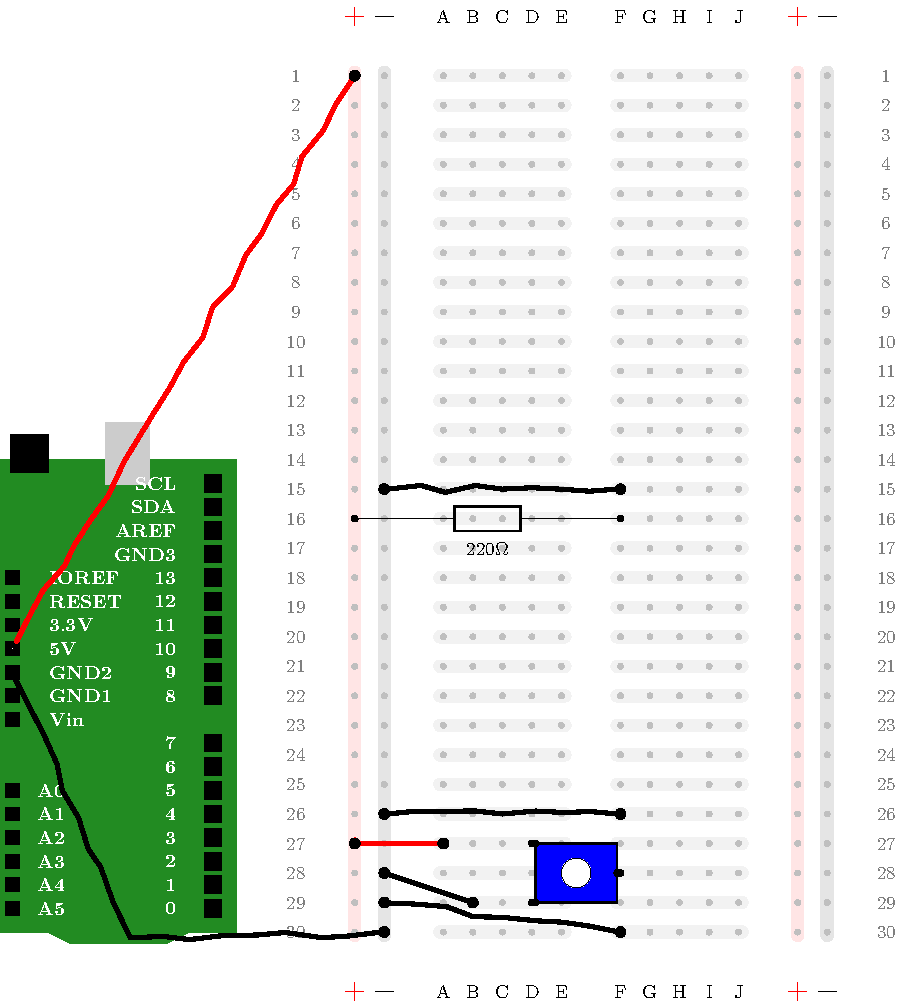
\includegraphics[width=0.95\textwidth]{kuvat/kuva20.pdf}

Kytketään sitten maat: rivi 26 oikea puoli maahan, rivi 30 oikea puoli maahan, ja rivi 15 oikea puoli maahan.

%%%%%%%%%%%%%%%%%%%

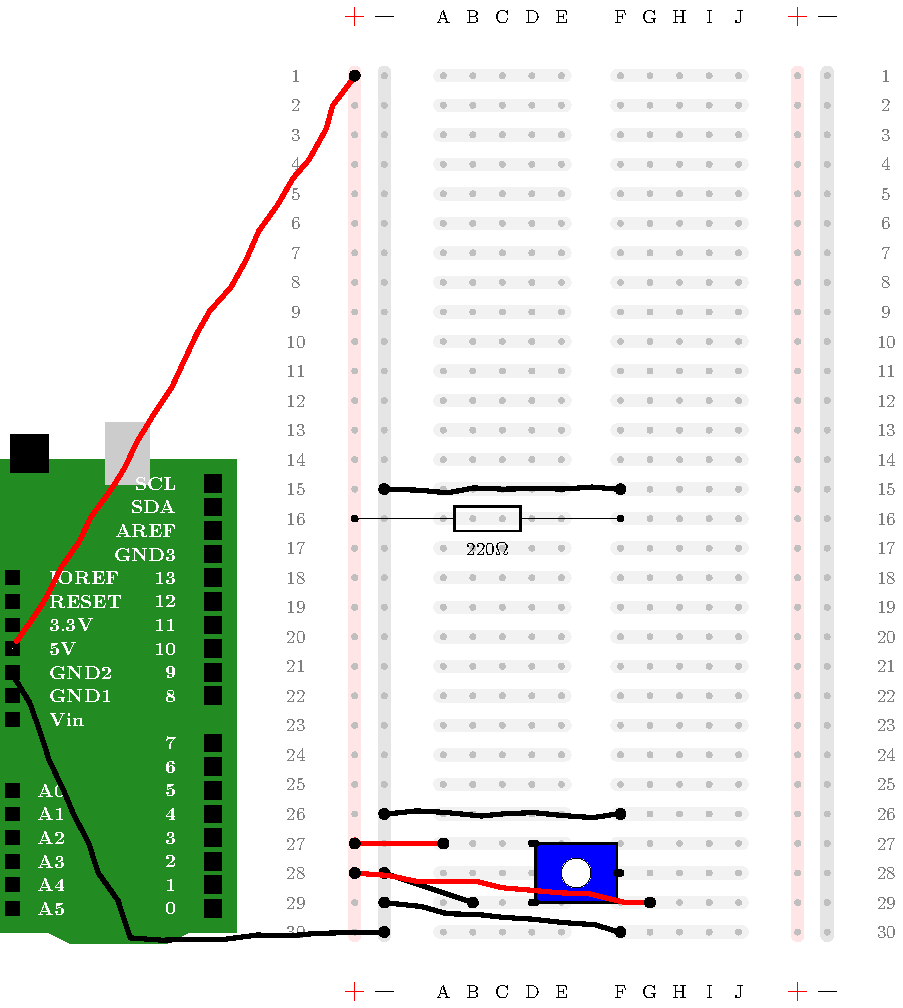
\includegraphics[width=0.95\textwidth]{kuvat/kuva21.pdf}

Kytketään sitten loput käyttöjännitteet: rivi 29 oikea puoli vasempaan plus-riviin (5V). 

%%%%%%%%%%%%%%%%%%

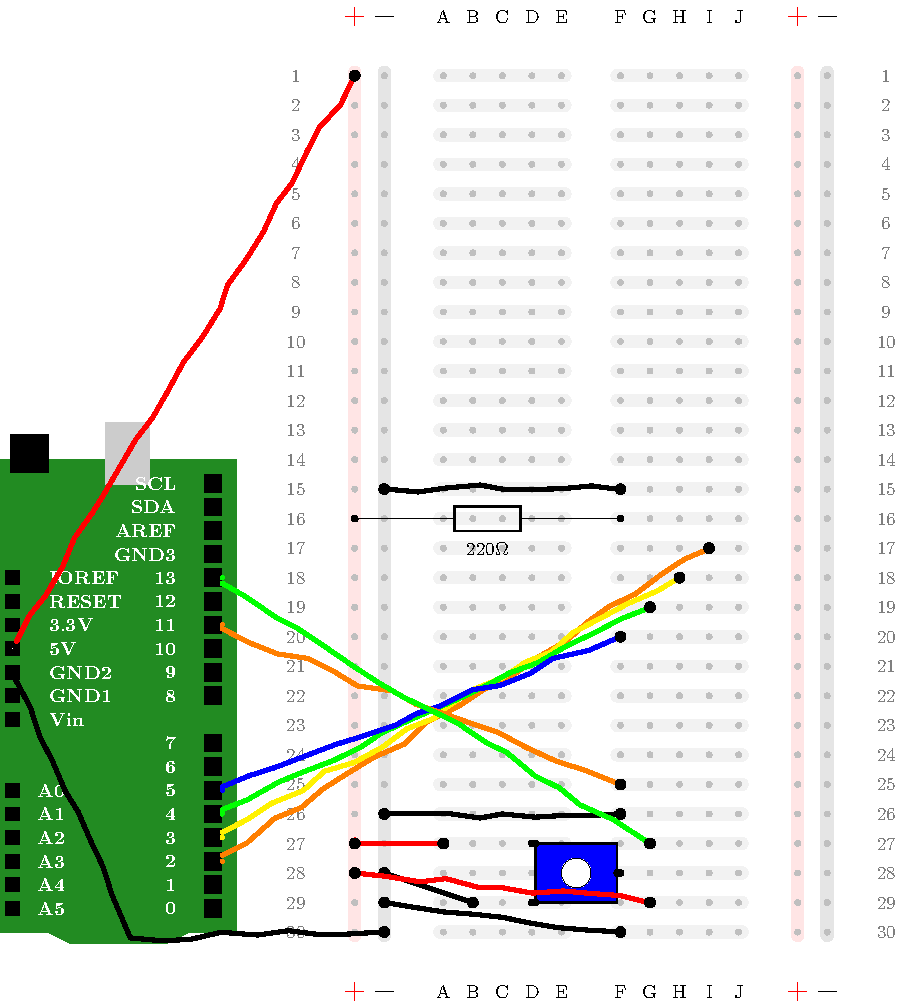
\includegraphics[width=0.95\textwidth]{kuvat/kuva22.pdf}

Kytketään Arduinon puolelta pinni 2 oikealle riville 17, pinni 3 oikealle riville 18, pinni 4 oikealle riville 19 ja pinni 5 oikealle riville 20. Lisäksi pinni 11 oikealle riville 25 ja pinni 13 oikealle riville 27. 

%%%%%%%%%%%%%%%%

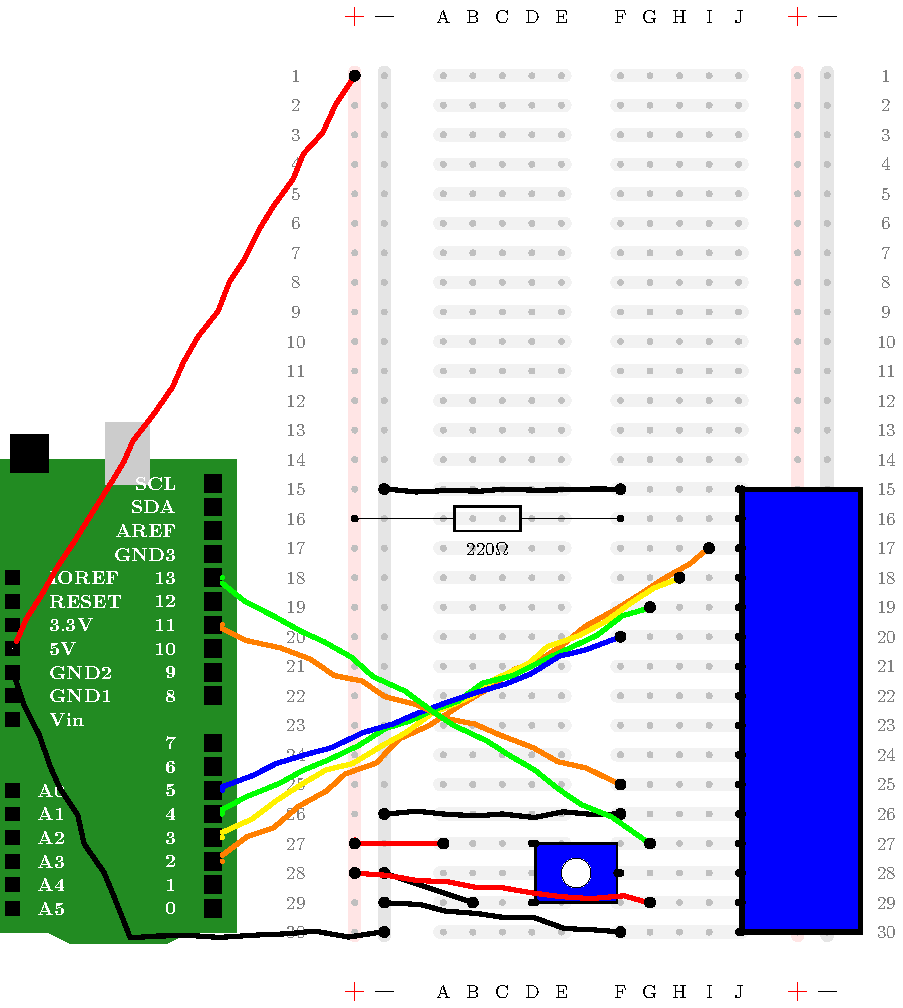
\includegraphics[width=0.9\textwidth]{kuvat/kuva23.pdf} \label{fig:lcd}

Viimeiseksi lisään LCD-näyttö kiinni pinneihin J15-J30.

\clearpage
Seuraavaksi koodataan Arduinolla näytölle tekstiä kahteen riviin. LCD-näytöllä on kaksi riviä, joiden pituus on 16 merkkiä riviä kohti. 

\begin{tcolorbox}[colback=white,title=Vinkkejä Arduinolla koodaamiseen!,colbacktitle=purple!90]
\begin{lstlisting}
// LCD-nayton kayttaminen onnistuu kirjaston avulla:
#include <LiquidCrystal.h> // Lisataan kirjasto 
// Arduinolle pitaa kertoa missa pinneissa naytto on kiinni:
LiquidCrystal lcd(13,11,5,4,3,2); // Digital Pinnit joissa kiinni

// Taman jalkeen naytolle voidaan tulostaa:
lcd.print("Viesti.");
// Naytto voidaan tyhjentaa
lcd.clear();
// Osoittimen paikkaa voidaan siirtaa:
lcd.setCursor(luku1, luku2);
// luku1 kertoo kuinka mones nayton osa (0-15)
// luku2 kertoo kumpi rivi, 0 = ylempi, 1 = alempi
\end{lstlisting}
\end{tcolorbox}

Kopioi koodi ja testaa, että saat näytölle näkyviin tekstin "Tervetuloa (Nimesi)". Jos näytöllä ei näy mitään, niin kokeile pyörittää potentiometria nupin avulla. Potentiometri säätää näytön kirkkautta. 

\begin{lstlisting}[numbers=none]
#include <LiquidCrystal.h> // Lisataan kirjasto 
LiquidCrystal lcd(13,11,5,4,3,2); // Digital Pinnit joissa kiinni

void setup() {
  lcd.begin(16,2); // Kaynnistetaan naytto
  lcd.print("Tervetuloa"); // Kirjoitetaan ekalle riville
}

void loop() {
  lcd.setCursor(0,1); // Siirrytaan toiselle riville
  lcd.print("Nimi"); // Kirjoita oma nimesi tahan
}
\end{lstlisting}

\clearpage
Seuraavaksi testataan, miten saadaan aikaan liikkuva teksti toiselle riville.

\begin{lstlisting}[numbers=none]
#include <LiquidCrystal.h> // Lisataan kirjasto 
LiquidCrystal lcd(13,11,5,4,3,2); // Digital Pinnit joissa kiinni

char * viesti = "Tanaan on ohjelmointipaiva.";

void setup() {
  lcd.begin(16,2);
  lcd.print("Tervetuloa");
}

void loop() {
  // Naytolle mahtuu 16 merkkia per rivi
  for (int letter = 0; letter <= strlen(viesti); letter++) {
    naytaViesti(0,letter);
  }
}

void naytaViesti(int printStart, int startLetter) {
  lcd.setCursor(printStart,1);
  for (int letter = startLetter; letter<=startLetter+15; letter++) {
    if (letter <=strlen(viesti)-1){
      lcd.print(viesti[letter]);
    } else {
      lcd.print(" ");
    }
  }
  lcd.print(" ");
  delay(300); // Lisataan viive, etta ehdimme lukea
}
\end{lstlisting}
Nyt alemmalla rivillä pitäisi liikkua määrittelemänne viesti! Voit muokata viestin liikkumisnopeutta muokkaamalla viivettä. Muokkaa koodia oman tervehdysten lähettämiseen!

\begin{tcolorbox}[colback=yellow!10, title={Koodaa!},colbacktitle=orange,breakable]
\begin{solution}
\begin{lstlisting}
#include <LiquidCrystal.h> // Lisataan kirjasto 
LiquidCrystal lcd(13,11,5,4,3,2); // Digital Pinnit joissa kiinni

// Tata muokkaamalla saadaan eri liikkuvia viesteja. 
char * viesti = "Tanaan on ohjelmointipaiva.";

void setup() {
  lcd.begin(16,2);
  lcd.print("Tervetuloa"); // Tata muokkaamalla ylarivi pysyy samana
}

void loop() {
  // Naytolle mahtuu 16 merkkia per rivi
  for (int letter = 0; letter <= strlen(viesti); letter++) {
    naytaViesti(0,letter);
  }
}

void naytaViesti(int printStart, int startLetter) {
  lcd.setCursor(printStart,1);
  for (int letter = startLetter; letter<=startLetter+15; letter++) {
    if (letter <=strlen(viesti)-1){
      lcd.print(viesti[letter]);
    } else {
      lcd.print(" ");
    }
  }
  lcd.print(" ");
  delay(300); // Lisataan viive, etta ehdimme lukea
}
\end{lstlisting}
\end{solution}
\end{tcolorbox}

\clearpage
\section{Lämpötilan mittaaminen ja näyttäminen näytöllä}
\begin{minipage}{0.5\textwidth}
\begin{tcolorbox}[colback=lime!10,title=Tarvikkeet, colbacktitle=green!10,coltitle=black]
\begin{itemize}
    \item Edellisen kohdan piiri rakennettuna
    \item Lämpötila-anturi (TMP36)
    \item Hyppylankoja
\end{itemize}
\end{tcolorbox}
\end{minipage}
\begin{minipage}{0.5\textwidth}
\begin{tcolorbox}[colback=blue!10,title=Piirin toiminta,colbacktitle=purple!90]
Mitataan huoneen lämpötila ja tulostetaan se LCD-näytölle.
\end{tcolorbox}
\end{minipage}

\begin{tcolorbox}[colback=red!10,colbacktitle=red,title=HUOM!]
Aina kun rakennat tai muutat piiriä, pidä Arduino irrotettuna tietokoneesta! 
\end{tcolorbox}

Lisätään lämpötila-anturi piiriin kuvan mukaisesti ja liitetään sen mittaus porttiin A0. 


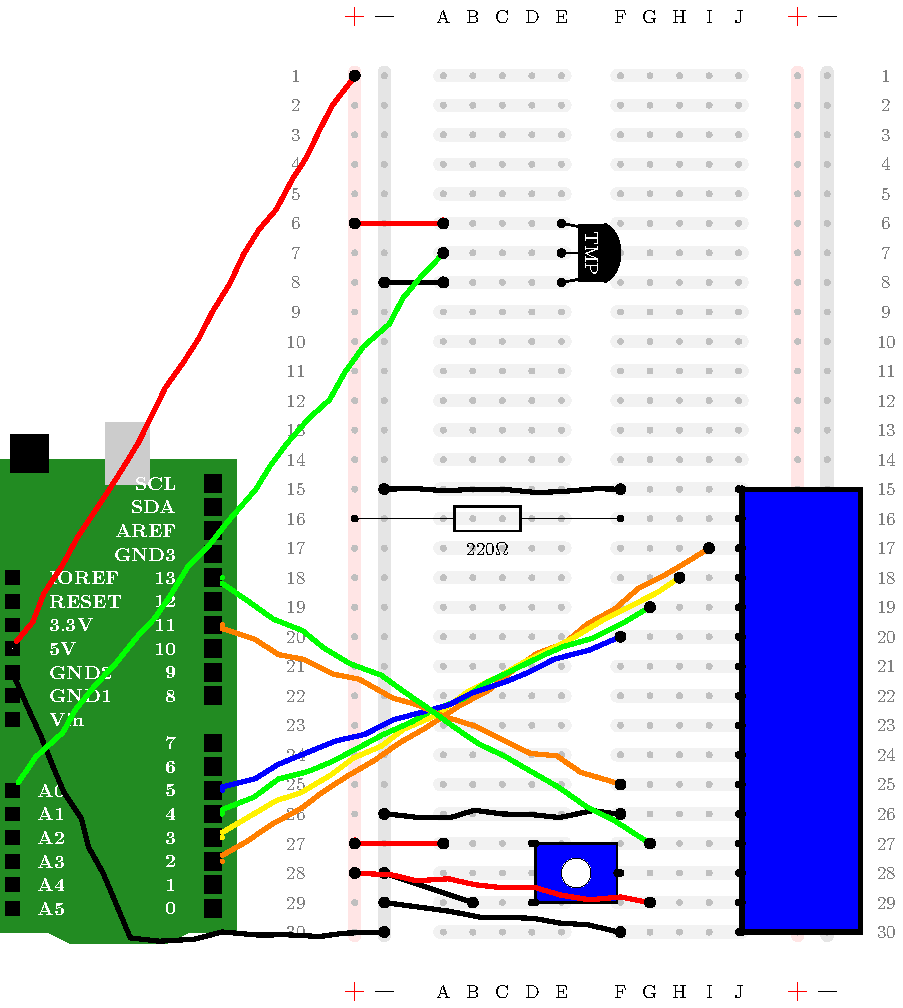
\includegraphics[width=0.8\textwidth]{kuvat/kuva24.pdf}

Kuten jo aiemmin, kun mittasimme lämpötilaa, voimme tehdä samoin nyt ja tulostaa lämpötilan serial portin sijaan näytölle.

\begin{lstlisting}[numbers=none]
#include <LiquidCrystal.h> // Lisataan kirjasto 
LiquidCrystal lcd(13,11,5,4,3,2); // Digital Pinnit joissa kiinni

void setup() {
  lcd.begin(16,2); // Aloitetaan kaytto
  lcd.print("Lampotila"); // Tulostetaan ensimmaiselle riville lampotila
}

void loop() {
  // Mitataan lampotila ja muunnetaan se asteiksi
  int sensorVal = analogRead(A0);
  float voltage = (sensorVal/1024.0)*5.0;
  float temp = (voltage-0.5)*100;
  // Ja tulostetaan se
  lcd.setCursor(0,1);
  lcd.print(temp);
  // Odotetaan arvojen paivittamisen valilla, etta luvut eivat hypi
  delay(1000);  
}
\end{lstlisting}
%%%%%%%%%%%%%%%%%%%%%%
\clearpage
\section{LCD-näyttö ja vaihtuvat viestit}
\begin{minipage}{0.5\textwidth}
\begin{tcolorbox}[colback=lime!10,title=Tarvikkeet, colbacktitle=green!10,coltitle=black]
\begin{itemize}
    \item Edellisen kohdan piiri rakennettuna
    \item Kaltevuusanturi
    \item Vastus 10k$\Omega$: 
\includegraphics[width=0.5\textwidth]{kuvat/10k.pdf}
\end{itemize}
\end{tcolorbox}
\end{minipage}
\begin{minipage}{0.5\textwidth}
\begin{tcolorbox}[colback=blue!10,title=Piirin toiminta,colbacktitle=purple!90]
Vaihdetaan LCD-näytön tekstiä kun havaitaan, että piiriä on kallistettu.
\end{tcolorbox}
\end{minipage}

\begin{tcolorbox}[colback=red!10,colbacktitle=red,title=HUOM!]
Aina kun rakennat tai muutat piiriä, pidä Arduino irrotettuna tietokoneesta! 
\end{tcolorbox}

\begin{tcolorbox}[title=Kaltevuusanturin kytkeminen,colback=blue!10,colbacktitle=purple!90]
Kaltevuusanturissa on neljä jalkaa, ja se vaatii kaksi riviä koekytkentälevystä. Kaltevuusanturi näyttää suorakulmaiselta laatikolta, jonka lähes neliönmuotoisella päällä lukee "UP" ja on nuoli ylös. Tämä rivi, jolla nuoli on, kytketään käyttöjännitteeseen ja toinen rivi kytketään vastuksen kautta maahan. Mittaustulos voidaan lukea samalta riviltä mille vastus on kytketty.  


\begin{tikzpicture}[scale=0.5]
\BREADBOARD (0,0) {5};
\draw[thick,fill=black] (D3.east) rectangle (E4.west) node[pos=0.5,color=white] {UP};
\draw (D3.east) to[short,*-*] (D3);
\draw (D4.east) to[short,*-*] (D4);
\draw (E3.west) to[short,*-*] (E3);
\draw (E4.west) to[short,*-*] (E4);

\draw[wire,red] (A3) to[short,*-o] ++(-7,0) node[left,black] {Käyttöjännite};
\draw[wire,blue] (A4) to[short,*-o] ++(-7,0) node[left,black] {Mittaus};

\end{tikzpicture}
\end{tcolorbox}

\begin{tcolorbox}[colback=white,title=Vinkkejä Arduinolla koodaamiseen!,colbacktitle=purple!90,breakable]
\begin{lstlisting}
// Satunnaisen luvun arpominen
int satunnainen = random(luku); //  satunnainen kokonaisluku valilta 0-annettu luku
// Ehtolause: ei yhta suuri kuin
luku1 != luku2
// Vaihtoehtoisia tapauksia
switch(luku) {
    case 0:
    // mita tehdaan jos luku on nolla
    break; // lopetetaan
    case 1: 
    // kun luku on 1
    break;
    // Lisaa case numero: riveja niin monta yhteensa kuin lukusi on ja kerro mita tehdaan, ja poistu sen jalkeen ulompaan koodiin break:n avulla
}
\end{lstlisting}
\end{tcolorbox}


Kytketään kaltevuusanturi ja vastus piiriin ja mitataan anturin antamaa arvoa pinnin 6 avulla. 

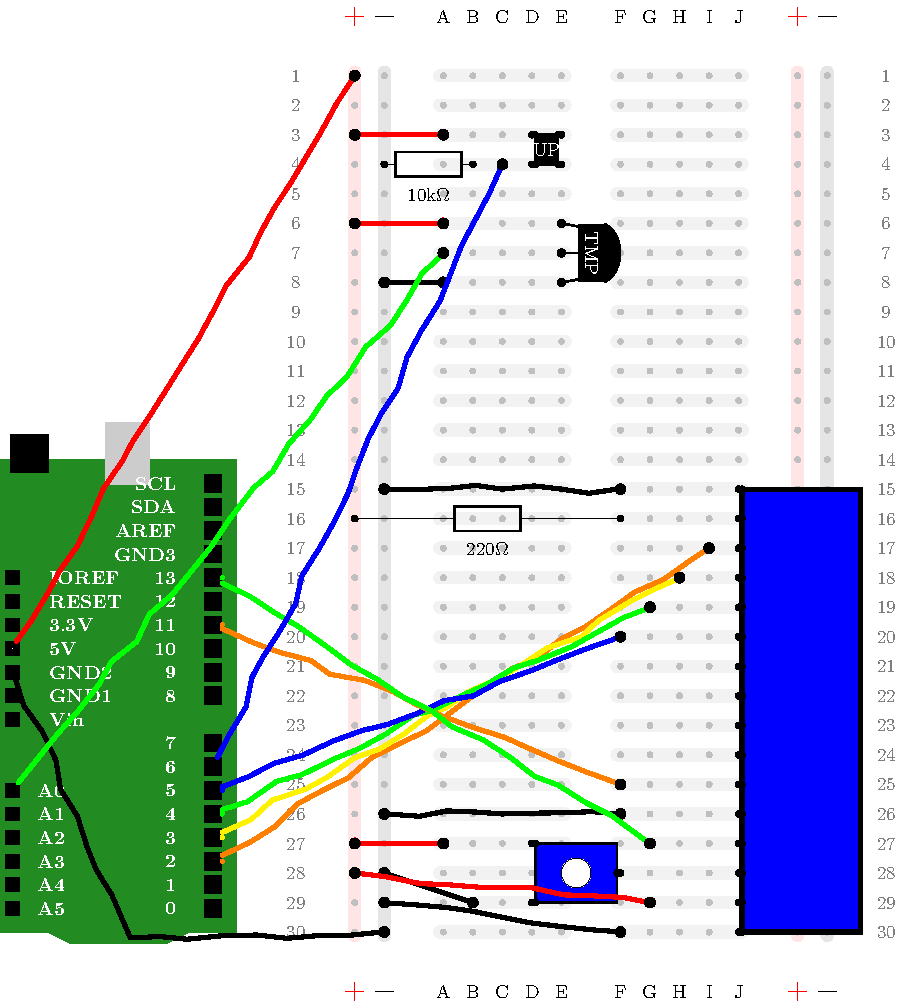
\includegraphics[width=0.8\textwidth]{kuvat/kuva25.pdf}


\clearpage
Lisätään koodiin kaltevuusanturin lukeminen ja koodataan muutama eri viesti näytöllä näytettäväksi.

\begin{lstlisting}[numbers=none]
#include <LiquidCrystal.h> // Lisataan kirjasto 
LiquidCrystal lcd(13,11,5,4,3,2); // Digital Pinnit joissa kiinni

int switchState = 0;
int prevSwitchState = 0;
int reply;

void setup() {
  lcd.begin(16,2);
  pinMode(6, INPUT); // Kaltevuusanturi pinnissa 6
  lcd.print("Hetken miete");
}

void loop() {
  // Luetaan kaltevuusanturin tila
  switchState = digitalRead(6);
  // Jos tila ei ole sama kuin edellinen tila, tehdaan asioita
  if (switchState != prevSwitchState) {
    if (switchState == LOW) {
      // Arvotaan mita naytetaan
      reply = random(4);
      // Tyhjennetaan naytto
      lcd.clear();
      // Asetetaan kursori ensimmaisen rivin alkuun
      lcd.setCursor(0,0);
      // Annetaan eri tapaukset ja mita tehdaan milloinkin
      switch(reply){
        case 0:
        lcd.print("Kytke ne");
        lcd.setCursor(0,1);
        lcd.print("sarjaan!");
        break;
        case 1:
        lcd.print("Kytke ne");
        lcd.setCursor(0,1);
        lcd.print("rinnan!");
        break;
        case 2:
        lcd.print("LEDit");
        lcd.setCursor(0,1);
        lcd.print("palaa!");
        break;
        case 3:
        lcd.print("Lampotila");
        lcd.setCursor(0,1);
        int sensorVal = analogRead(A0);
        float volt = (sensorVal/1024.0)*5.0;
        float temp = (volt-0.5)*100;
        lcd.print(temp);
        break;
      }
    }
  } 
  // Viimekseksi tallennetaan edelliseksi tilaksi nykyinen tila
  prevSwitchState = switchState;
}
\end{lstlisting}

Testaa toiminta nostamalla sitä. Heiluta varovasti koekytkentälevyä, niin että viestit vaihtuvat näytöllä.

\begin{tcolorbox}[title=Haaste!,colback=teal!10,colbacktitle=teal!90]
Muuta koodia niin, että saat aikaa mystisen kasipallon! Eli, koodaa 8 eri vastausta kysymyksiin, jotka saat esiin ravistamalla kevyesti koekytkentälevyä.
\end{tcolorbox}

\begin{tcolorbox}[colback=yellow!10, title={Koodaa!},colbacktitle=orange,breakable]
\begin{solution}
\begin{lstlisting}
#include <LiquidCrystal.h> // Lisataan kirjasto 
LiquidCrystal lcd(13,11,5,4,3,2); // Digital Pinnit joissa kiinni

int switchState = 0;
int prevSwitchState = 0;
int reply;

void setup() {
  lcd.begin(16,2);
  pinMode(6, INPUT); // Kaltevuusanturi pinnissa 6
  lcd.print("Mystinen");
  lcd.setCursor(0,1);
  lcd.print("Kasipallo!");
}

void loop() {
  // Luetaan kaltevuusanturin tila
  switchState = digitalRead(6);
  // Jos tila ei ole sama kuin edellinen tila, tehdaan asioita
  if (switchState != prevSwitchState) {
    if (switchState == LOW) {
      // Arvotaan mita naytetaan
      reply = random(8);
      switch(reply){
        case 0:
        lcd.clear();
        lcd.setCursor(0,0);
        lcd.print("Tietokone sanoo");
        lcd.setCursor(0,1);
        lcd.print("ei.");
        break;
        case 1:
        lcd.clear();
        lcd.setCursor(0,0);
        lcd.print("Tottakai!");
        break;
        case 2:
        lcd.clear();
        lcd.setCursor(0,0);
        lcd.print("Ei missaan");
        lcd.setCursor(0,1);
        lcd.print("nimessa");
        break;
        case 3:
        lcd.clear();
        lcd.setCursor(0,0);
        lcd.print("Kuuma!");
        break;
        case 4:
        lcd.clear();
        lcd.setCursor(0,0);
        lcd.print("Kylma!");
        break;
        case 5:
        lcd.clear();
        lcd.setCursor(0,0);
        lcd.print("Mahdollisesti!");
        break;
        case 6:
        lcd.clear();
        lcd.setCursor(0,1);
        lcd.print("Huomenna!");
        case 7:
        lcd.clear();
        lcd.setCursor(0,0);
        lcd.print("Lampotila");
        lcd.setCursor(0,1);
        int sensorVal = analogRead(A0);
        float volt = (sensorVal/1024.0)*5.0;
        float temp = (volt-0.5)*100;
        lcd.print(temp);
        break;
      }
    }
  } 
  // Viimekseksi tallennetaan edelliseksi tilaksi nykyinen tila
  prevSwitchState = switchState;
}
\end{lstlisting}
Keskustelua voi nostaa esimerkiksi siitä, kuinka satunnainen random() oikeastaan on. 

Kannattaa muistaa myös, että Arduinossa on piirissä reset-nappula tietokone-liitännen vieressä, jos haluat palauttaa koodin takaisin alkupisteeseen.
\end{solution}
\end{tcolorbox}